\begin{figure*}
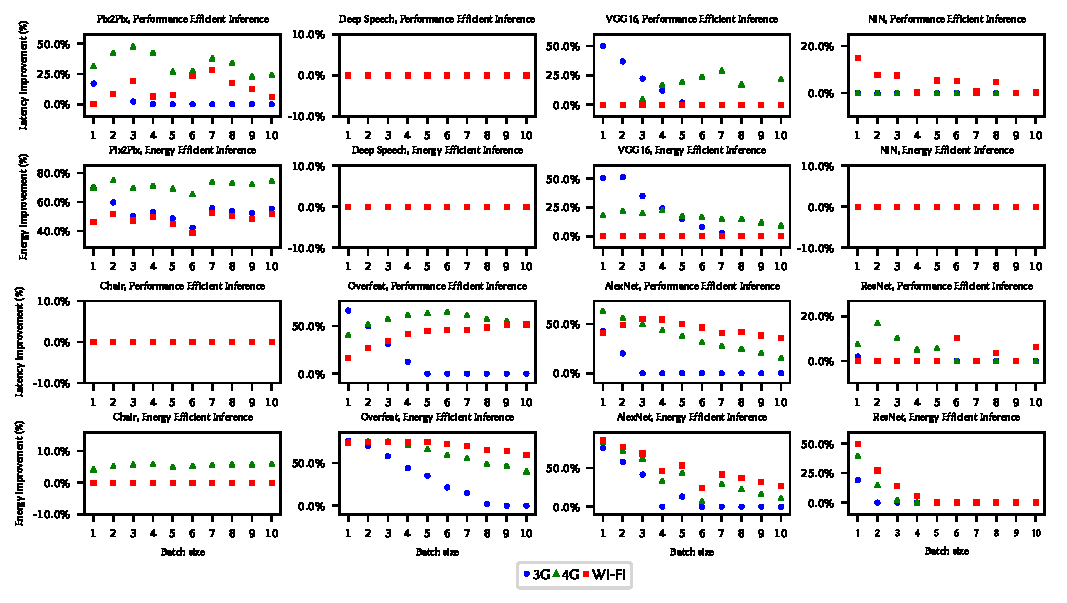
\includegraphics{inference_results}
\caption{Latency and energy improvements for different batch sizes during inference.}
\label{inference_results}
\end{figure*}

\begin{figure*}
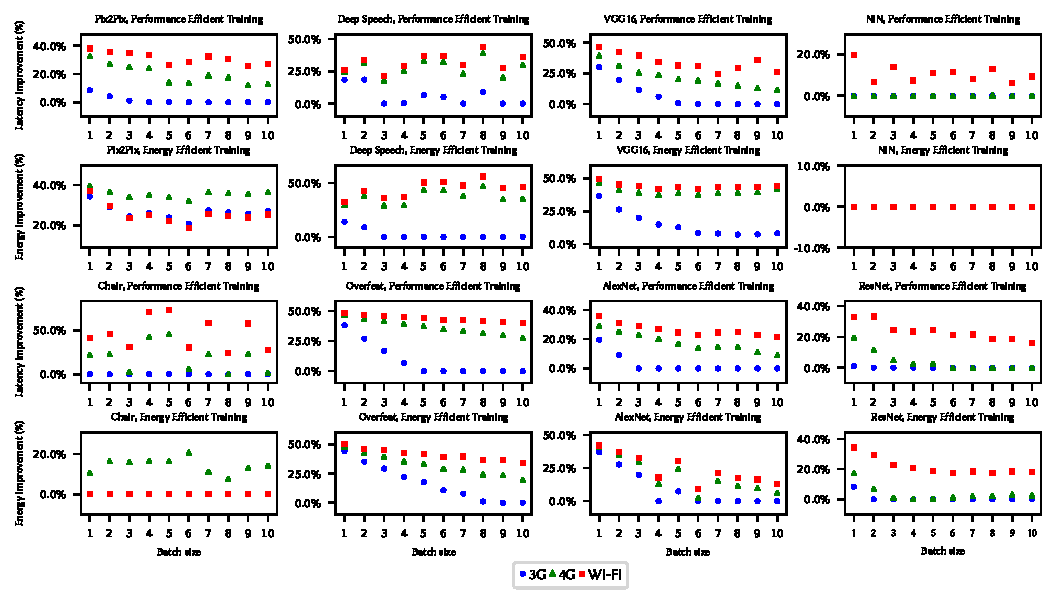
\includegraphics[width=\linewidth]{training_results}
\caption{Latency and energy improvements for different batch sizes during training.}
\label{training_results}
\end{figure*}

\section{Evaluation}

\subsection{Deep Architecture Benchmarks}

Since the architecture of neural networks depends on the type of the application, we have chosen three common application types of DNNs:

\begin{enumerate}
\item \textbf{Discriminative neural networks} are a class of models in machine learning for modeling the conditional probability distribution $P(y|x)$. This class generally is used in classification and regression tasks. AlexNet\cite{AlexNet}, OverFeat\cite{OverFeat}, VGG16\cite{VGG16}, Deep Speech\cite{DeepSpeech}, ResNet\cite{ResNet}, and NiN\cite{NiN} are well-known discriminative models we use as benchmarks in this experiment. Except Deep Speech, used for speech recognition, all other benchmarks are used in image classification tasks. 

\item \textbf{Generative neural networks} model the joint probability distribution $P(x,y)$, allowing generation of new samples. These networks have applications in Computer Vision~\cite{GAN} and Robotics~\cite{DeepVisual}, which can be deployed on a mobile device. Chair~\cite{Chair} is a generative model we use as benchmark in this work.
\item \textbf{Autoencoders} are another class of neural networks used to learn a representation for a data set. Their applications are image reconstruction, image to image translation, and denoising to name a few. Mobile robots can be equipped with autoencoders to be used in their computer vision tasks. We use Pix2Pix~\cite{Pix2Pix}, as a benchmark from this class.
\end{enumerate}

\begin{table}
\caption{Benchmark Specifications}
\centering
\begin{adjustbox}{center}
     %\begin{adjustbox}{center}
        \begin{tabular}{|c|c|c|}
        \hline
        \textbf Type & \textbf Model & \textbf Layers \\                
            \hline
            \multirow{4}{*}{Discriminative} & \multicolumn{1}{c}{AlexNet} & \multicolumn{1}{|c|}{21} \\\cline{2-3}
            & \multicolumn{1}{c}{OverFeat} & \multicolumn{1}{|c|}{14} \\\cline{2-3}
            & \multicolumn{1}{c}{Deep Speech} & \multicolumn{1}{|c|}{10} \\\cline{2-3}
            & \multicolumn{1}{c}{ResNet} & \multicolumn{1}{|c|}{70} \\\cline{2-3}
            & \multicolumn{1}{c}{VGG16} & \multicolumn{1}{|c|}{37} \\\cline{2-3}
            & \multicolumn{1}{c}{NiN} & \multicolumn{1}{|c|}{29} \\\hline
           Generative & Chair & 10 \\                \hline
            Autoencoder &  Pix2Pix & 32 \\                \hline
        \end{tabular}
     \end{adjustbox}
%     \vspace{ - 05 mm}

\label{benchmarks}
\end{table}

\begin{table}[h]
	\caption{Mobile networks specifications in the U.S.} 
	\centering 
	\begin{tabular}{|c|c|c|c|} \hline
	\textbf{Param.} & \textbf{3G} & \textbf{4G} & \textbf{Wi-Fi} \\ \hline
	Download speed (Mpbs)	& 	2.0275 	&	13.76 	&	54.97 \\ \hline
	Upload speed (Mbps)	&	1.1		&	5.85	&	18.88 \\ \hline
$\alpha_u$ (mW/Mpbs)	& 868.98	& 438.39	&	283.17    \\ \hline
$\alpha_d$ (mW/Mpbs)	 & 122.12 	& 51.97	&	137.01        \\ \hline
$\beta$ (mW)	& 817.88	& 1288.04	&	132.86            \\ \hline
\end{tabular}
\label{table:network_parameters} 
\end{table}

\subsection{Mobile and Server Setup}
We used Jetson TX2 module developed by NVIDIA\textsuperscript{\textregistered}~\cite{JetsonTX2}, a fair representative of mobile computation power as our mobile device. This module enables efficient implementation of DNN applications used in products such as robots, drones, and smart cameras. It is equipped with NVIDIA Pascal\textregistered GPU with 256 CUDA cores and a shared 8~GB 128~bit LPDDR4 memory between GPU and CPU. To measure the power consumption of the mobile platform, we used INA226 power sensor~\cite{INA226}. 

NVIDIA\textsuperscript{\textregistered} Tesla\textsuperscript{\textregistered} K40C~\cite{TeslaGPU} with 12~GB memory serves as our server GPU. The computation capability of this device is more than one order of magnitude compared to our mobile device. 
% TODO: Should I mention that we are not measuring the server power?
% TODO: Should we make the rows of the two tables the same? System? 
% TODO: textregistered sign in table 
% Reference on the table title?

\subsection{Communication Parameters}
To model the communication between platforms, we used the average download and upload speed of mobile Internet~\cite{MobNet, Speedtest} for different networks (3G, 4G and Wi-Fi) as shown in Table~\ref{table:network_parameters}.


The communication power for download ($P_d$) and upload ($P_u$) is dependent on the network throughput ($t_d$ and $t_u$). Comprehensive examinations in~\cite{4GLTE} indicates that uplink and downlink power can be modeled with linear equations (Eq.~\ref{eq:power_model_eq}) fairly accurate with less than 6\% error rate. Table~\ref{table:network_parameters} shows the parameter values of this equation for different networks. 

\begin{equation}
\begin{split}
P_u = \alpha_u t_u + \beta \\
P_d = \alpha_d t_d + \beta \label{eq:power_model_eq}
  \end{split}
\end{equation}


